\documentclass[final, 16pt]{beamer}
% poster
\usepackage[size=custom, width=121.92, height=91.44]{beamerposter}
% common stuff
\usepackage{graphicx}
\usepackage{hyperref}
\usepackage{booktabs}
\usepackage{amsmath}
\usepackage{caption}
\usepackage{subcaption}
\usepackage{array}
\usepackage{xparse}
\usepackage{wrapfig}
\usepackage{xspace}
% necessary acronyms
\def\ie{\textit{i.e.}\xspace}
\def\eg{\textit{e.g.}\xspace}
\def\etc{\textit{etc.}\xspace}
\def\etal{\textit{et al.}\xspace}
\def\cf{\textit{cf.}\xspace}
% font
\usefonttheme{serif}
\setbeamerfont{block title}{size=\Large, series=\bfseries}
\setbeamerfont{headline title}{size=\fontsize{64}{0pt}\selectfont, series=\bfseries}
\setbeamerfont{headline author}{size=\large, series=\bfseries}
% main color
\definecolor{theme-1}{HTML}{1e3a8a} % #1e3a8a
\definecolor{theme-2}{HTML}{14b8a6} % #14b8a6
\definecolor{theme-3}{HTML}{f5f5f4} % #f5f5f4
\definecolor{theme-4}{HTML}{fafaf9} % #fafaf9
% set color
\setbeamercolor{block title}{fg=theme-3, bg=theme-1}
\setbeamercolor{headline title}{fg=theme-4, fg=theme-1}
\setbeamercolor{footnote}{fg=theme-1}
\setbeamercolor{footnote mark}{fg=theme-1}

% \setbeamerfont{footnote}{size=\small}

\let\oldfootnoterule\footnoterule
\renewcommand{\footnoterule}{\color{theme-1}{\oldfootnoterule}}
% linespace
\usepackage{setspace}
\setstretch{1.25}
% size
\setlength{\paperwidth}{48in}
\setlength{\paperheight}{36in}
\setlength{\footnotesep}{1cm}
\newlength{\sepwidth}
\newlength{\colwidth}
\newlength{\twocolwidth}
\newlength{\contentwidth}
\newlength{\contentheight}
\newlength{\marginwidth}

\usepackage{calc}
\setlength{\marginwidth}{0.5in}
\setlength{\contentwidth}{\paperwidth - 2\marginwidth}
\setlength{\contentheight}{\paperheight - 3in}
\setlength{\sepwidth}{0.005\contentwidth}
% 4 columns
\setlength{\colwidth}{(\contentwidth - 3\sepwidth) / 4}
\setlength{\twocolwidth}{\colwidth + \sepwidth + \colwidth}
% empty spacer column
\NewDocumentCommand{\separatorcolumn}{}{\begin{column}{\sepwidth}\end{column}}
\NewDocumentCommand{\margincolumn}{}{\begin{column}{\marginwidth}\end{column}}
% itemize style to dots
\setbeamertemplate{itemize items}[circle]
% top head template
\setbeamertemplate{headline}{
  \begin{beamercolorbox}{headline}
    \usebeamerfont{headline}
    \vskip0.5in
    \centering
    {\usebeamerfont{headline title}\usebeamercolor[fg]{headline title}\inserttitle\\[0.5ex]}
    {\usebeamerfont{headline author}\usebeamercolor[fg]{headline author}\insertauthor\\[1ex]} % author is not allowed.
    \ifbeamercolorempty[bg]{headline rule}{}{
      \begin{beamercolorbox}[wd=\paperwidth,colsep=0.5ex]{headline rule}\end{beamercolorbox}
    }
  \end{beamercolorbox}
}
\usepackage{tikz}
\usetikzlibrary{calc}
\NewDocumentCommand{\ensuremargin}{}{
  \begin{tikzpicture}[remember picture,overlay]
    \draw[black] ($(current page.north west) - (0, 1.5in)$) -- ($(current page.north east) - (0, 1.5in)$);
    \draw[black] ($(current page.south west) + (0, 1.5in)$) -- ($(current page.south east) + (0, 1.5in)$);
    \draw[black] ($(current page.north west) + (1in, 0)$) -- ($(current page.south west) + (1in, 0)$);
    \draw[black] ($(current page.north east) - (1in, 0)$) -- ($(current page.south east) - (1in, 0)$);
  \end{tikzpicture}
}
% header helper
\usepackage{xhfill}
\NewDocumentCommand{\header}{m O{1.5em}}{\vspace{#2}\begingroup\usebeamercolor[bg]{block title}\scshape\Large#1\par\vspace{-0.45\baselineskip}\hrulefill\endgroup}
\NewDocumentCommand{\subheader}{m}{\begingroup\usebeamercolor[bg]{block title}\bfseries\large#1\par\endgroup}

% multicol
\usepackage{multicol}
% hanging indent
\usepackage{hanging}
% numbered figure and table
\setbeamertemplate{caption}[numbered]
% metadata
\title{Undulatory Swimming: A Topological and Computational Model}
\author{Dobromir Iliev, Anish Goyal, \& Ricardo Guardado \\\normalfont The Gwinnett School of Math, Science, and Technology}
% bullet
\newenvironment{myitemize}
    {\begin{itemize}[leftmargin=5.5mm]}
    {\end{itemize}}
% redefine block
\let\block=\undefined
\let\endblock=\undefined
\usepackage[most]{tcolorbox}
\newtcolorbox{block}[1]{enhanced, colback=white, colframe=theme-1!50, colbacktitle=theme-1, coltitle=white, fonttitle=\bfseries, title=\Large#1, boxrule=1pt, boxsep=1.5em, breakable, sharpish corners, bottomrule=0.5em, toptitle=-0.75em, bottomtitle=-0.75em}
% microtype
\usepackage[activate={true,nocompatibility},final]{microtype}

% remove navigation
\setbeamertemplate{navigation symbols}{}
% make vfill work in beamer columns
\usepackage{etoolbox}
\let\oldcolumn\column
\let\oldendcolumn\endcolumn
\RenewDocumentEnvironment{column}{m O{\contentheight - 2.7in}}{%
  \oldcolumn{#1}%
  \minipage[c][#2][s]{\columnwidth}
}{\endminipage\oldendcolumn}

\begin{document}
\setlength{\columnsep}{50pt}

\begin{frame}[t]
\centering
\vspace*{-0.5cm}
\begin{columns}[t]
\margincolumn

\fontsize{22}{26}\selectfont

\begin{column}{\colwidth}
  \fontsize{22}{24}\selectfont

  \begin{block}{Background}
    \header{Literature Review}[0pt]

    Undulatory swimming, characterized by wave-like movements propagating along the body, is a prevalent mode of locomotion in aquatic organisms, including fish and marine mammals. This form of propulsion aalows aquatic organisms to navigate through water with \textbf{minimal energy expenditure} and maintain homeostasis. This is accomplished through the use of complex synaptic transmission pathways, which coordinate muscle contractions that generate the propulsive forces they need to swim. Previous studies have shown that the number of fired neurons is directly correlated to the current flow through these synaptic channels that are responsible for sending electrical signals for muscle movement. One such case study is the \textbf{Zebrafish}, a creature with highly specialized neurotransmitters along its spine to spur dorsal muscles and generate torque. Additionally, Zebrafish generate rheumatic swimming without sensory input due to central pattern generators in their brains. This makes them ideal to study for locomotion because outside stimuli will \emph{not} pose a confounding effect on their movement. Because of these unique properties, Zebrafish ECG data can serve as a framework to optimize undulatory propulsion systems.

    \begin{multicols}{2}
      \begin{figure}[H]
        \centering
        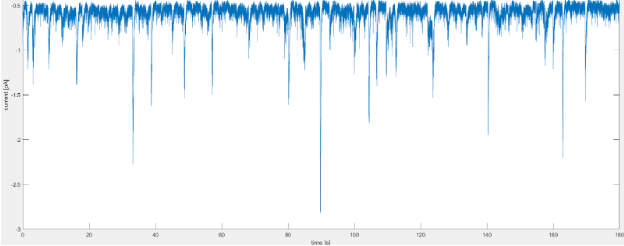
\includegraphics[width=0.95\linewidth, height=0.65\linewidth]{img/ECG_Data.png}
        \caption{Sample Zebrafish ECG data}
        \label{fig:ecg-data}
      \end{figure}
      
      \begin{figure}[H]
        \centering
        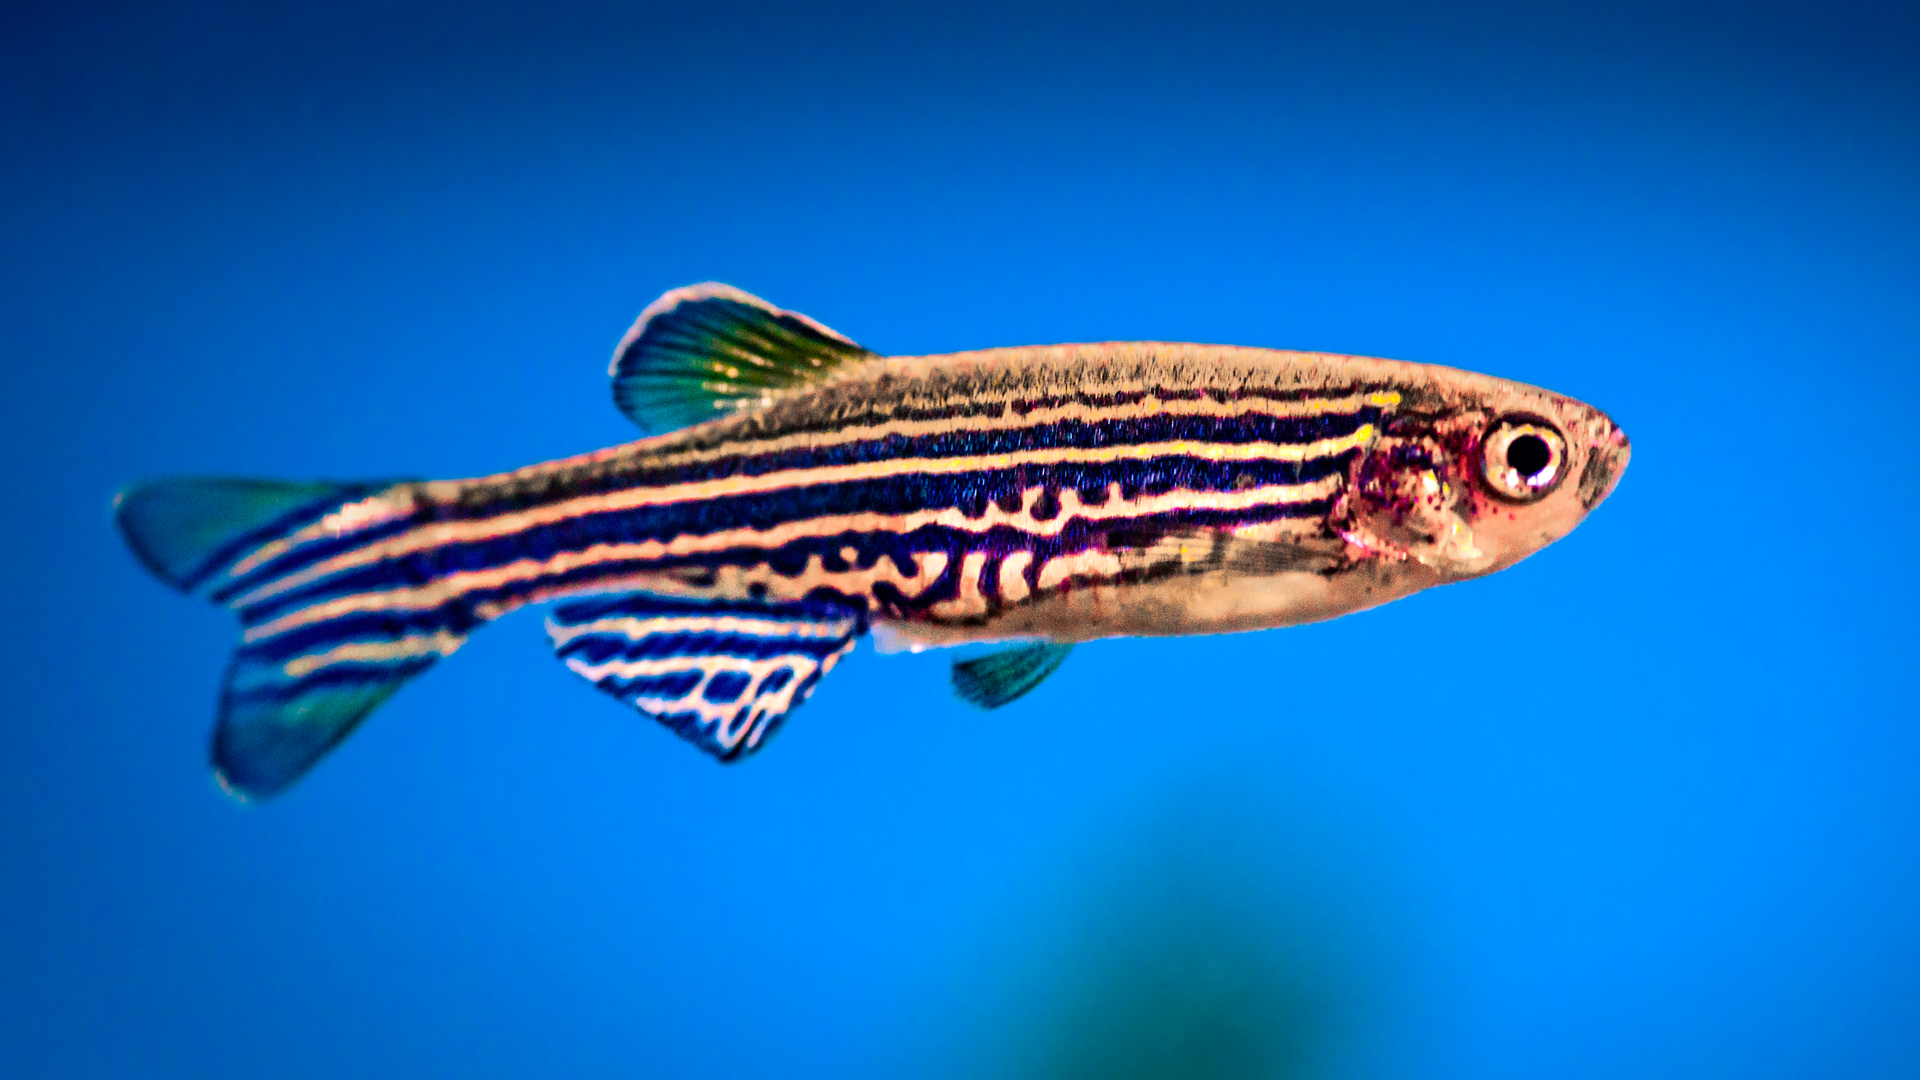
\includegraphics[width=0.95\linewidth]{img/Zebrafish.png}
        \caption{Picture of a Zebrafish \\ Sourced from www.bcs.mit.edu}
        \label{fig:zebrafish}
      \end{figure}
    \end{multicols}

    Scientists and engineers alike have determined that it is theoretically possible to design propulsion systems that mimic the neuromuscular pathways of aquatic organisms like the Zebrafish. These aptly-called \textbf{biomimetic propulsion systems} have the potential to be more efficient than traditional propulsion systems because they are \textbf{self-regulating} in respose to environmental stimuli. Additionally, fluid dynamics and mesh topology are critical in enhancing a biomimetic-powered submersible's energy efficiency even further. Modern oceanic topological models are generated using either queues or parallelization, as implementing both simultaneously causes a mismatch in object size initialization, leading to excessive computational overload.

    \header{Problem Statement}[0pt]

    A comprehensive model that integrates neuromuscular control mechanisms and fluid dynamics into a unified design has yet to be realized. Current submersibles do not fully utilize \textbf{biological locomotion} or implement \textbf{priority queues} in generating their topological models. This limitation hinders their ability to navigate complex underwater terrain and adapt to changing environmental conditions. Moreover, as climate change impacts ocean conditions, there is a growing need for improved ecosystem monitoring and mapping of the ocean floor for deep-sea exploration.

    This leads us to the fundamental problem we wanted to solve: \emph{How can we develop a propulsion system that integrates the complex neuromuscular control mechanisms of Zebrafish with fluid dynamics to mimic natural propulsion more efficiently than traditional systems?} Such a system could not only enhance the maneuverability and efficiency of underwater vehicles but also \textbf{revolutionize ecosystem monitoring, mapping of the ocean floor, and deep-sea exploration}. 

  \end{block}

  \begin{block}{Target Planning}
    \header{Engineering Goal}[0pt]

    Our engineering goal is to create an optimized submersible powered by a novel biomimetic propulsion system and topological model to help scientists conduct climate research and map the ocean. Specifically, the submersible should:

    \begin{itemize}
      \item Have a functional 3D structure that minimizes water forces
      \item Mimic the neurology of Zebrafish to create an energy-efficent propulsion system
    \end{itemize}

    \header{Evaluation Hypotheses}[0pt]
    
    We needed to come up with a way to evaluate our project on completion. Ultimately, we decided to \textbf{combine} \emph{the Scientific Method} and \emph{the Engineering Design Process} to create evaluation hypotheses that would gauge the effectiveness of our final product:

    \begin{itemize}
    \item \textbf{Null Hypothesis:} Both the biomimetic propulsion system and topological model do not differ in energy efficiency compared to a traditional propulsion system.
    \item \textbf{Experimental hypothesis:} The biomimetic propulsion system and topological model will both exhibit \emph{statistically significant} \footnote{ \emph{We will use the standard convention for statistical significance ($p < 0.05$) in this project.}} differences in energy efficiency compared to a traditional propulsion system.
    \end{itemize}

  \end{block}

\end{column}

\separatorcolumn

\begin{column}{\twocolwidth}

  \begin{block}{Engineering Methodology}

    \header{Pre-planning}[0pt]

    \vspace{0.5cm}

    \begin{minipage}{0.24\linewidth}
      \subheader{Constraints}
      \begin{itemize}
        \item Restricted in 3D printing techniques
        \item Testing outside of a lab environment
        \item Unoptimal motor driver and power sensor specs
        \item Time frame of 4 weeks
        \item Limited budget of \$100
      \end{itemize}
    \end{minipage}\hfill%
    \begin{minipage}{0.72\linewidth}
      \subheader{Materials}
      \begin{multicols}{3}
      \begin{description}
        \item[Distilled Water] 1 gallon
        \item[Arduino Nano] 1
        \item[Meter-long water container] 1
        \item[Breadboard Jumper Cables] 30
        \item[L985 Motor] 1 
        \item[Mini Breadboard] 1
        \item[Raspberry PI 4B] 1
        \item[Stepper motors] 2
        \item[USB 3.0 Hub] 1
        \item[Ovonic LiPo battery] 1 
        \item[INA219 Sensor] 1
        \item[TPU resin] 400 grams
        \item[Duct tape] 1
        \item[Stop watch] 1
        \item[Electrical cables] 20
      \end{description}
    \end{multicols}
    \end{minipage}

    \header{Experimental Setup}

    \begin{minipage}[t]{0.48\linewidth}
      \subheader{Topological Model}
      \begin{enumerate}
        \item Fill a large bucket with water, approximately one meter long.
        \item Place the control model, a block of equivalent mass, at one end of the bucket.
        \item Place the optimized model next to the control.
        \item Connect both models to the opened version of the proposed propulsion system, with the optimized propulsion system not in effect.
        \item Start a timer as soon as both models are connected to the propulsion system.
        \item Record the time it takes for each model to reach the other end of the bucket.
        \item Obtain feedback on the energy expenditure when each model reaches the other end.
        \item Document the energy expenditure in kilowatt-hours for each model.
      \end{enumerate}
    \end{minipage}\hfill%
    \begin{minipage}[t]{0.48\linewidth}
      \subheader{Neurological Model}

      \begin{enumerate}
        \item Same as step one for the topological model.
        \item Place the model into the larger container.
        \item Connect to the closed loop system with ROS using PuTTY.
        \item Call the command to start the model.
        \item Stop the model after it traverses one meter.
        \item Record the power draw from the INA219 sensor.
        \item Repeat for fifty iterations.
        \item Repeat the same procedurce, instead calling open loop control through the motor directly with SSH.
      \end{enumerate}
    \end{minipage}

    \vspace*{1cm}

    \header{System Architecture}[0pt]

    \begin{minipage}[t]{0.48\linewidth}
      \subheader{Beta I}

      Beta I was the initial prototype of our submersible, which utilized Navier-Stokes

       \begin{wrapfigure}{r}{0.35\linewidth}
        \centering
        \vspace*{-0.5cm}
        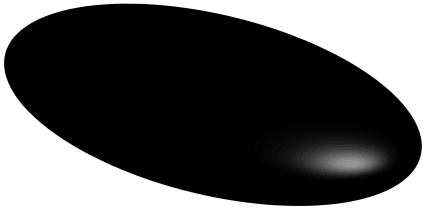
\includegraphics[scale=0.35]{img/Topological_Model.png}
        \caption{Picture of Beta I}
        \label{fig:beta-i}
      \end{wrapfigure}

      equations to construct optimized vector field graphs based on parameters such as water viscosity, time step, and water density. To convert the vector fields into a printable CAD model, we used MATLAB's Simulink tool to convert the field graphs into a vtb file and imported it into OnShape.

      \begin{figure}[H]
        \centering
        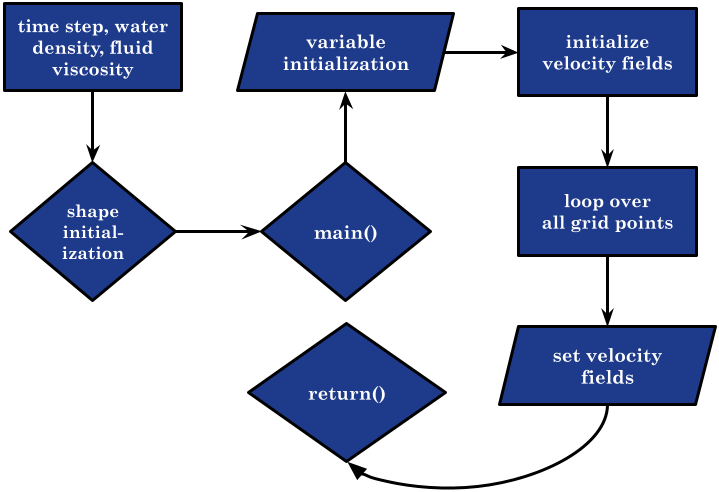
\includegraphics[width=0.8\linewidth, height=0.50\linewidth]{img/Topological_Flow_Chart.png}
        \caption{A flowchart of the topological processing}
        \label{fig:topological-flow-chart}
      \end{figure}

    \end{minipage}\hfill%
    \begin{minipage}[t]{0.48\linewidth}
      \subheader{Beta II}

      Beta II of our model incorporates \textbf{octree indexing}, which offers several advantages over traditional XYZ graphing methods. It partitions 3D space into hierarchical, smaller sections, providing a more organized and compact representation of spatial data. This indexing allows for logarithmic time complexity in search operations, making it highly scalable. 
      
      \begin{wrapfigure}{r}{0.35\linewidth}
        \centering
        \vspace*{-1.5cm}
        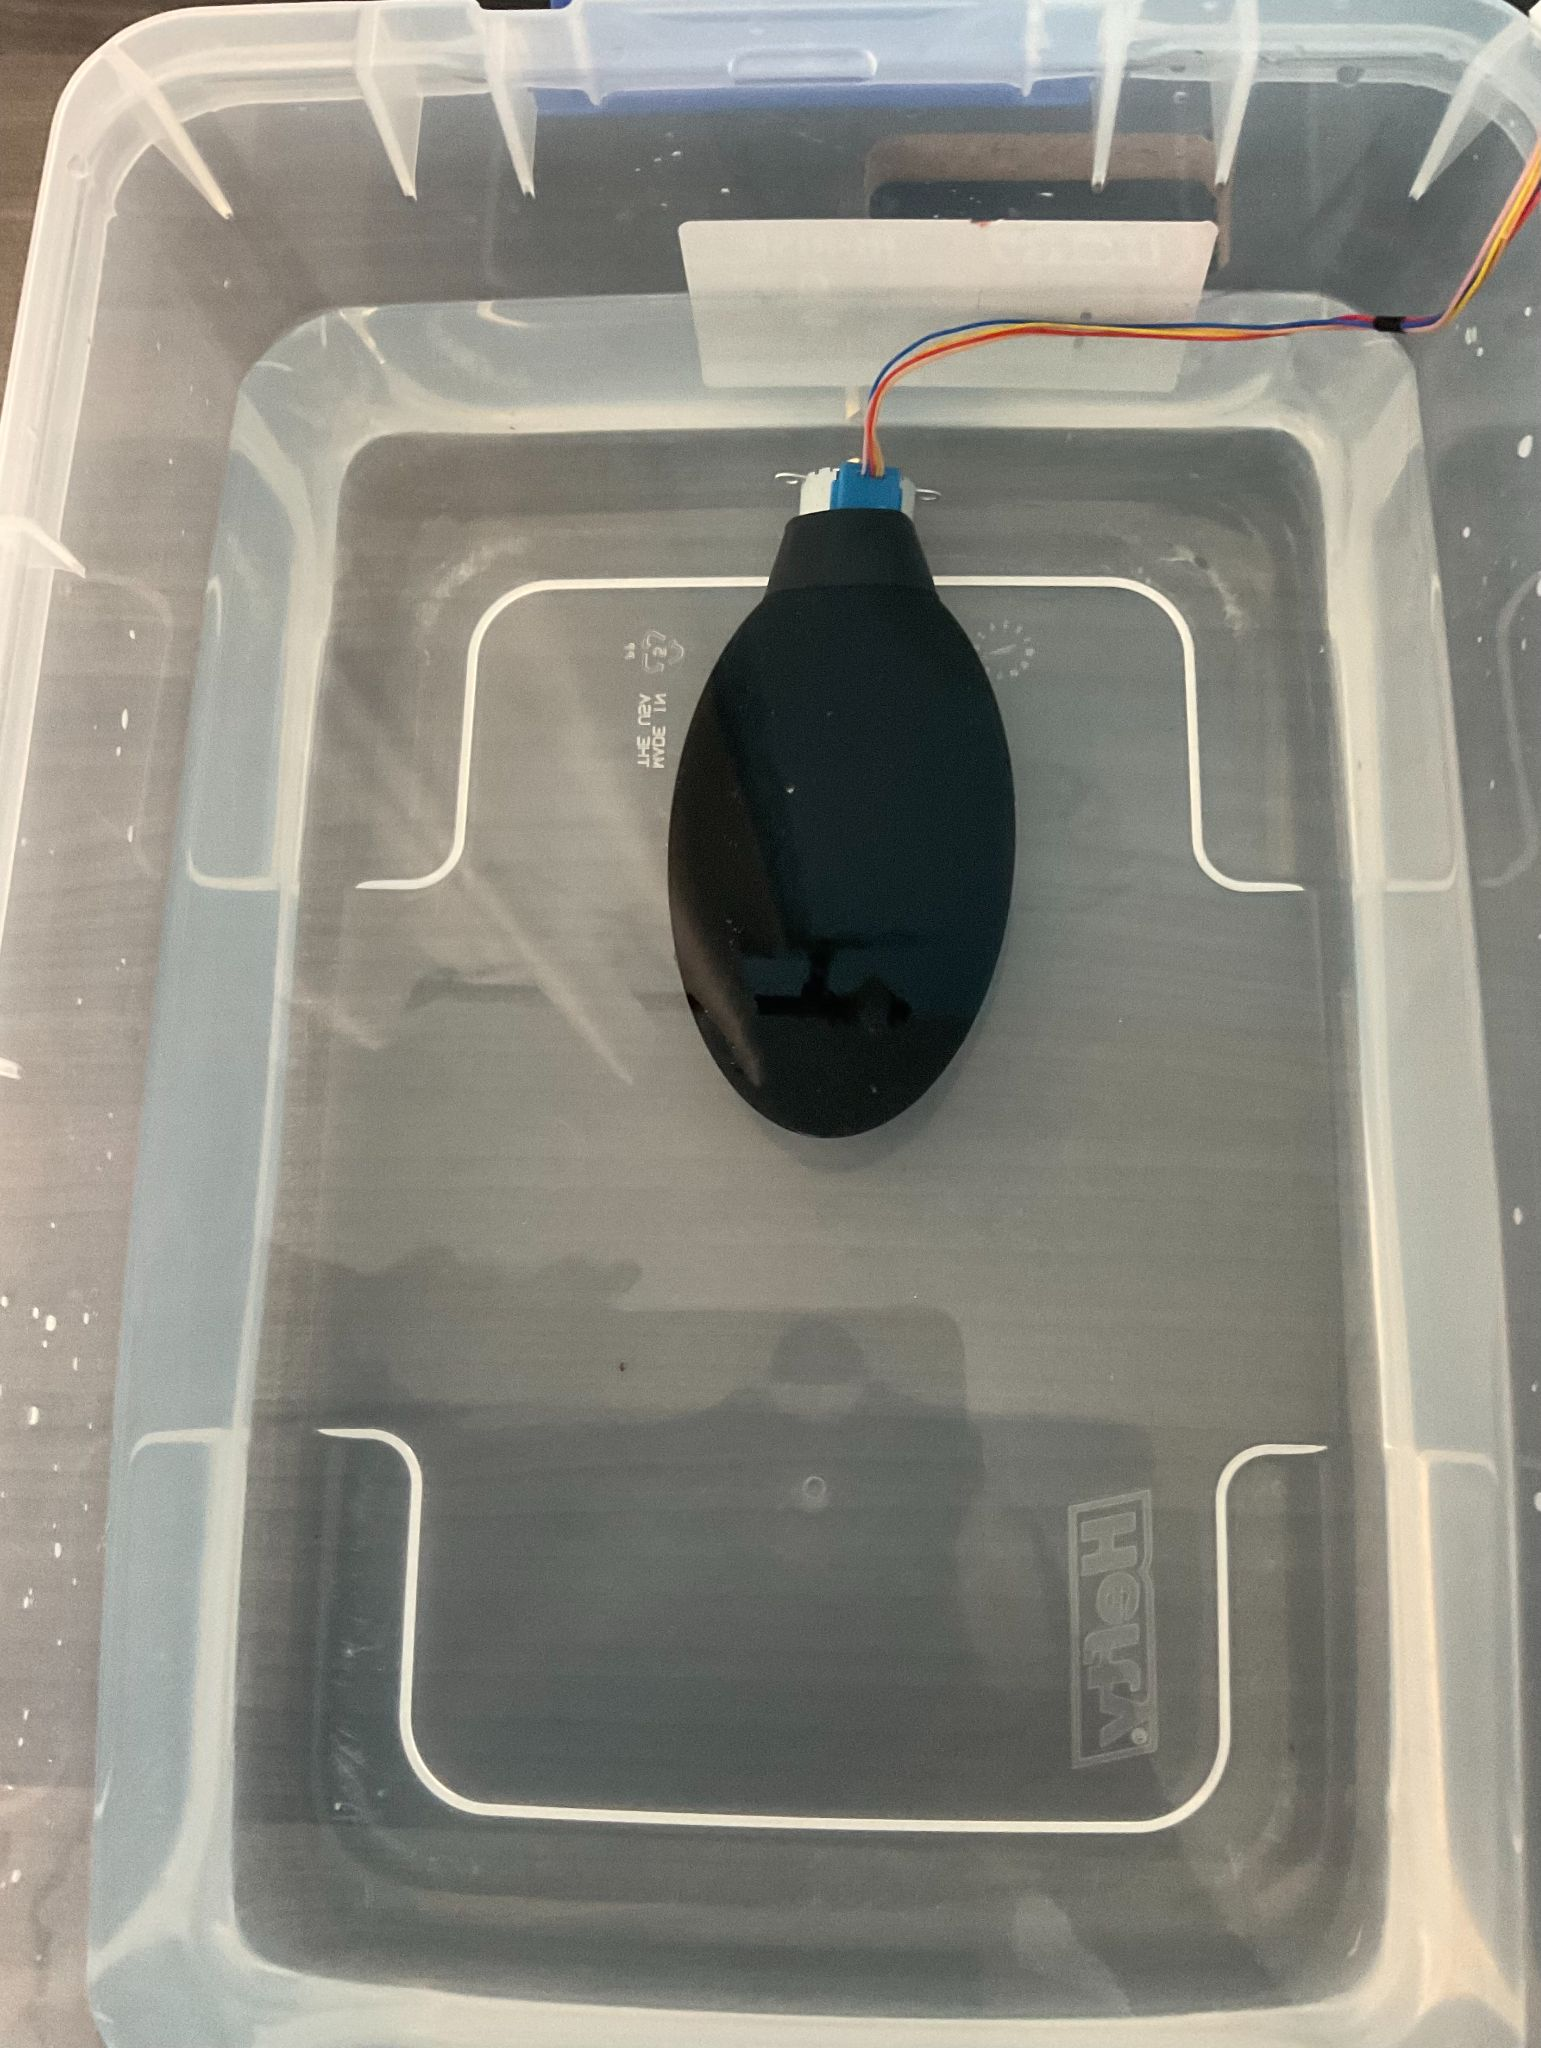
\includegraphics[scale=0.15, height=0.30\textwidth, width=0.30\textwidth]{img/Beta_II.jpg}
        \caption{Picture of Beta II}
        \label{fig:beta-ii}
      \end{wrapfigure}

      It also enables efficient updates, typically involving only modifying a small part of the tree, unlike XYZ graphing, which may require reprocessing and reindexing an entire data set. Additionally, octree indexing significantly reduces the number of calculations needed to determine visible surfaces, enhancing overall efficiency. We have since \textbf{printed and tested} Beta II, making it our final product.

      \begin{figure}[H]
        \centering
        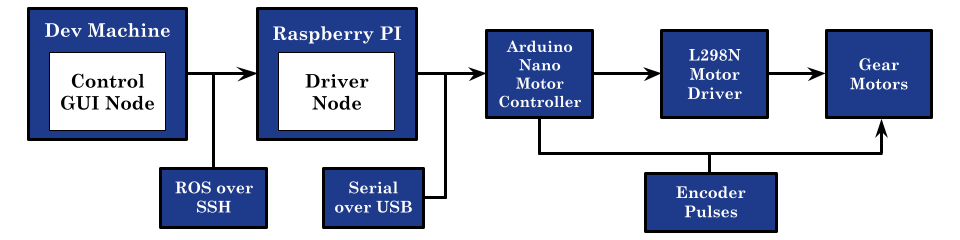
\includegraphics[width=0.95\linewidth]{img/Circuit_Flow_Chart.png}
        \caption{A flowchart of the circuitry}
        \label{fig:circuit-flow-chart}
      \end{figure}
    \end{minipage}

  \end{block}

  \begin{multicols}{2}
  \begin{block}{Data Collection \& Validation Testing}
      \begin{multicols}{2}
      \begin{figure}
       \centering
        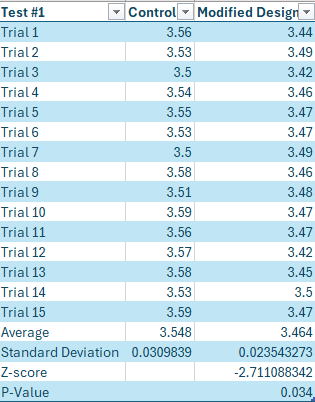
\includegraphics[scale=1.50]{img/Topological_Model_Table.png}
        \caption{Topological model data}
        \label{fig:topological-table}
      \end{figure}
      \begin{figure}
        \centering
        \vspace*{0.25cm}
         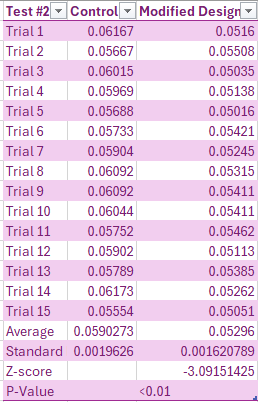
\includegraphics[scale=1.50]{img/Propulsion_Model_Table.png}
         \caption{Propulsional model data}
         \label{fig:propulsion-table}
       \end{figure}
      \end{multicols}
  \end{block}
  \begin{block}{Neurological Model}
    \begin{figure}
      \centering
      \vspace*{0.25cm}
       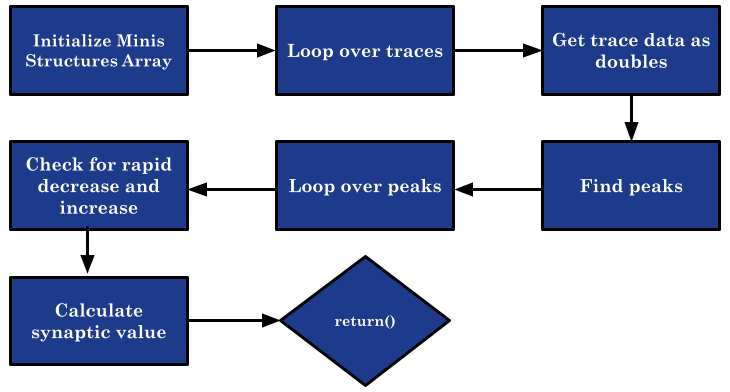
\includegraphics[height=0.65\linewidth, width=0.9\linewidth]{img/Neurological_Model.png}
       \caption{Neurological model framework}
       \label{fig:neurological-model}
     \end{figure}
  \end{block}
\end{multicols}
\end{column}

\separatorcolumn

\begin{column}{\colwidth}
  \begin{block}{Statistical Analysis}
    \vspace*{-1.1cm}
    \header{Testing for Significance}

    We conducted a \textbf{left-tailed z-test}, utilizing known values of standard mean and deviation, across all 15 trials for each model.

    \vspace*{-1.1cm}
    \header{Model Performance Benchmarks}

    \vspace*{-1.3cm}
    \begin{multicols}{2}
      \begin{figure}[H]
        \centering
        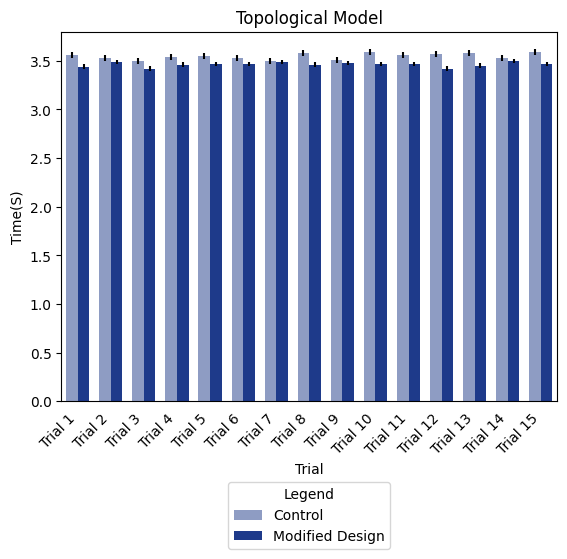
\includegraphics[width=1.05\linewidth, height=1.25\linewidth]{img/Topological_Model_Benchmark.png}
        \caption{Topological model benchmark}
        \label{fig:topological-model-benchmark}
      \end{figure}
      
      \begin{figure}[H]
        
        \centering
        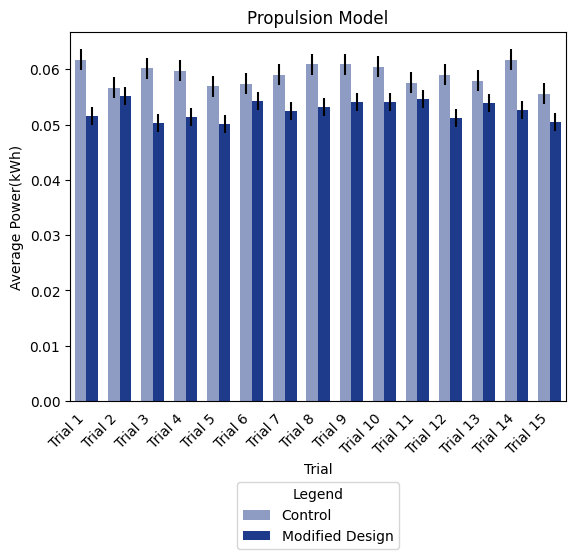
\includegraphics[width=1.05\linewidth, height=1.25\linewidth]{img/Propulsion_Model_Benchmark.png}
        \caption{Propulsion model benchmark}
        \label{fig:propulsion-model-benchmark}
      \end{figure}
    \end{multicols}

  \end{block}

  \begin{block}{Conclusions}
    \header{Interpretation of Results}[0pt]

    The topological and propulsion model $z$-scores of -2.71 and -3.09 correspond to $p$-values of 0.003 and 0.001, respectively. Since neither p-value is above 0.05, \textbf{we can reject the null hypothesis} that neither the biomimetic propulsion system nor topological model would differ in energy efficiency compared to a traditional propulsion system. 
    
    \header{Implications}[0pt]
    
    \textbf{The implications of our work are far-reaching.} By utilizing an innovative design and novel approach for locomotion, we were able to create \textbf{a highly efficient propulsion system} and \textbf{novel topological model} without the need for expensive components or complex manufacturing processes. This technology, coupled with the \textbf{scalable nature} of biomimetic propulsion systems, could alter how humans explore the ocean moving forward. Google is exploring the use of submersibles and LIDAR to automate ocean topography mapping rather than satellite imagery capturing the ocean serface, which is too reflective/too difficult for light to penetrate.
    \begin{wrapfigure}{r}{0.55\linewidth}
      \centering
      \vspace*{-0.5cm}
      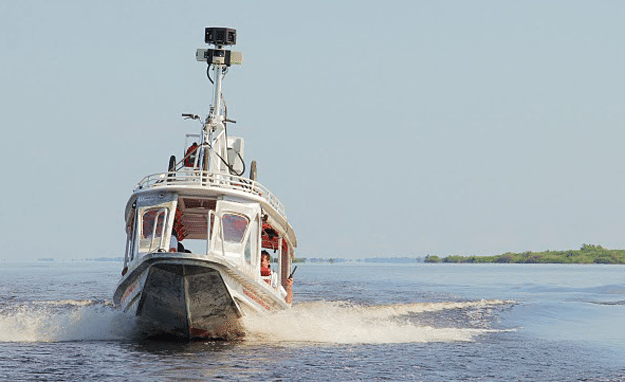
\includegraphics[width=\linewidth, height=0.4\linewidth]{img/Street_View_Boat.png}
      \caption{Picture of Google's "Street View" boat \\ Sourced from www.gcaptain.com}
      \label{fig:street-view-boat}
    \end{wrapfigure} 
    Other companies could potentially send out multiple unmanned vehicles simultaneously, efficiently covering large areas of the ocean floor for research and exploration purposes.

    \header{Future Work}[0pt]

    \begin{description}
      \item[LIDAR Technology] Our ROS driver pairs well with existing LIDAR technology.
      \item[Camera Visioning] JeVois camera microprocessors with a Generic Object Detection Tensor are a cheap solution for automated movement/collision detection.
      \item[FPGA Chips] Reduces communication latency down to \emph{microseconds}.    
    \end{description}

  \end{block}

  \begin{block}{Key References}

    \begin{hangparas}{.25in}{1}
      Borrill, C. (2023, April). Chrisb2/pi\_ina219: Raspberry Pi Python library for voltage and current sensors using the INA219. GitHub. https://github.com/chrisb2/pi\_ina219
    \end{hangparas}

    \begin{hangparas}{.25in}{1}
      Evgrafov, A. (2004, December). Topology optimization of Navier-Stokes equations. https://www.semanticscholar.org/paper/Topology-Optimization-of-Navier-Stokes-Equations-Evgrafov/c07ff8c44d5a24a9e6ff7dfec6ae8a42d93b054d 
    \end{hangparas}

    \begin{hangparas}{.25in}{1}
      Queralta, J. P., Yuhong, F., Salomaa, L., Qingqing, L., Gia, T. N., Zou, Z., Tenunen, H., \& Westerlund, T. (2019, October). FPGA-based architecture for a low-cost 3D lidar design. https://ieeexplore.ieee.org/abstract/document/8956928 
    \end{hangparas}

    \begin{hangparas}{.25in}{1}
      Roussel, Y., Gaudreau, S. F., Kacer, E. R., Sengupta, M., \& Bui, T. V. (2021). Modeling spinal locomotor circuits for movements in developing zebrafish. eLife, 10, e67453. https://doi.org/10.7554/eLife.67453
    \end{hangparas}

  \end{block}
\end{column}

\margincolumn
\end{columns}

\vspace*{6cm}
\tikz {
  \draw ($(current page.south west)!1!(current page.south east)$) node {\textbf{Unless otherwise stated, all charts, graphs, photos, and diagrams are products of the student researchers.}};
}
\end{frame}
\end{document}